\tikzset{every picture/.style={line width=0.75pt}} %set default line width to 0.75pt        

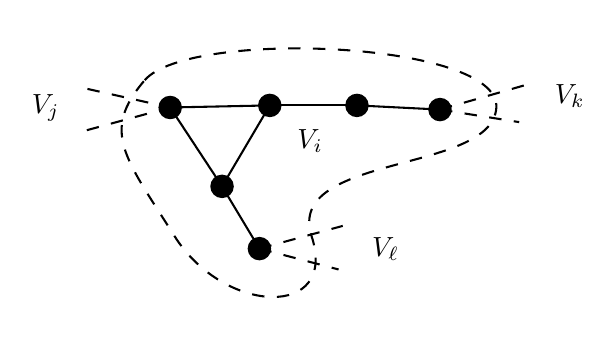
\begin{tikzpicture}[x=0.75pt,y=0.75pt,yscale=-1,xscale=1]
%uncomment if require: \path (0,507); %set diagram left start at 0, and has height of 507

%Shape: Circle [id:dp6074038045104917] 
\draw  [fill={rgb, 255:red, 0; green, 0; blue, 0 }  ,fill opacity=1 ] (90,184.15) .. controls (90,181.31) and (92.31,179) .. (95.15,179) .. controls (97.99,179) and (100.3,181.31) .. (100.3,184.15) .. controls (100.3,186.99) and (97.99,189.3) .. (95.15,189.3) .. controls (92.31,189.3) and (90,186.99) .. (90,184.15) -- cycle ;
%Shape: Circle [id:dp4763210712255822] 
\draw  [fill={rgb, 255:red, 0; green, 0; blue, 0 }  ,fill opacity=1 ] (138,183.15) .. controls (138,180.31) and (140.31,178) .. (143.15,178) .. controls (145.99,178) and (148.3,180.31) .. (148.3,183.15) .. controls (148.3,185.99) and (145.99,188.3) .. (143.15,188.3) .. controls (140.31,188.3) and (138,185.99) .. (138,183.15) -- cycle ;
%Shape: Circle [id:dp3853217426553297] 
\draw  [fill={rgb, 255:red, 0; green, 0; blue, 0 }  ,fill opacity=1 ] (115,222.15) .. controls (115,219.31) and (117.31,217) .. (120.15,217) .. controls (122.99,217) and (125.3,219.31) .. (125.3,222.15) .. controls (125.3,224.99) and (122.99,227.3) .. (120.15,227.3) .. controls (117.31,227.3) and (115,224.99) .. (115,222.15) -- cycle ;
%Shape: Circle [id:dp28821193699150127] 

\draw  [fill={rgb, 255:red, 0; green, 0; blue, 0 }  ,fill opacity=1 ] (180,183.15) .. controls (180,180.31) and (182.31,178) .. (185.15,178) .. controls (187.99,178) and (190.3,180.31) .. (190.3,183.15) .. controls (190.3,185.99) and (187.99,188.3) .. (185.15,188.3) .. controls (182.31,188.3) and (180,185.99) .. (180,183.15) -- cycle ;
%Shape: Circle [id:dp7382778383957265] 
\draw  [fill={rgb, 255:red, 0; green, 0; blue, 0 }  ,fill opacity=1 ] (133,252.15) .. controls (133,249.31) and (135.31,247) .. (138.15,247) .. controls (140.99,247) and (143.3,249.31) .. (143.3,252.15) .. controls (143.3,254.99) and (140.99,257.3) .. (138.15,257.3) .. controls (135.31,257.3) and (133,254.99) .. (133,252.15) -- cycle ;
%Straight Lines [id:da4581338904755592] 
\draw    (95.15,184.15) -- (143.15,183.15) ;
%Straight Lines [id:da30615918485309224] 
\draw    (95.15,184.15) -- (120.15,222.15) ;
%Straight Lines [id:da7970372677901666] 
\draw    (120.15,222.15) -- (143.15,183.15) ;
%Straight Lines [id:da6163192951001095] 
\draw    (143.15,183.15) -- (185.15,183.15) ;
%Shape: Circle [id:dp28499605169790954] 

\draw  [fill={rgb, 255:red, 0; green, 0; blue, 0 }  ,fill opacity=1 ] (220,185.15) .. controls (220,182.31) and (222.31,180) .. (225.15,180) .. controls (227.99,180) and (230.3,182.31) .. (230.3,185.15) .. controls (230.3,187.99) and (227.99,190.3) .. (225.15,190.3) .. controls (222.31,190.3) and (220,187.99) .. (220,185.15) -- cycle ;
%Straight Lines [id:da0792931196376595] 
\draw    (185.15,183.15) -- (225.15,185.15) ;
%Straight Lines [id:da8976761166666631] 
\draw    (120.15,222.15) -- (138.15,252.15) ;
%Straight Lines [id:da4659786097379426] 
\draw  [dash pattern={on 4.5pt off 4.5pt}]  (138.15,252.15) -- (178.3,241.2) ;
%Straight Lines [id:da817963072200574] 
\draw  [dash pattern={on 4.5pt off 4.5pt}]  (138.15,252.15) -- (176.3,262.2) ;
%Straight Lines [id:da03883979984290231] 
\draw  [dash pattern={on 4.5pt off 4.5pt}]  (55,195.1) -- (95.15,184.15) ;
%Straight Lines [id:da453819115170471] 
\draw  [dash pattern={on 4.5pt off 4.5pt}]  (55.3,175.2) -- (95.15,184.15) ;

%Straight Lines [id:da12564542484112884] 
\draw  [dash pattern={on 4.5pt off 4.5pt}]  (225.15,185.15) -- (270.3,172.2) ;
%Straight Lines [id:da47514468204336124] 
\draw  [dash pattern={on 4.5pt off 4.5pt}]  (225.15,185.15) -- (263.3,191.2) ;
%Shape: Polygon Curved [id:ds4531772485698] 
\draw  [dash pattern={on 4.5pt off 4.5pt}] (82.93,170.97) .. controls (104.3,146.2) and (254.22,152.17) .. (252.3,184.2) .. controls (250.37,216.22) and (150.3,206.2) .. (163.3,246.2) .. controls (176.3,286.2) and (121.3,284.2) .. (97.3,246.2) .. controls (73.3,208.2) and (61.55,195.75) .. (82.93,170.97) -- cycle ;

\draw (155,193.4) node [anchor=north west][inner sep=0.75pt]    {$V_{i}$};
% Text Node
% Text Node
\draw (27,176.4) node [anchor=north west][inner sep=0.75pt]    {$V_{j}$};
% Text Node
\draw (279,171.4) node [anchor=north west][inner sep=0.75pt]    {$V_{k}$};
% Text Node
\draw (191,245.4) node [anchor=north west][inner sep=0.75pt]    {$V_{\ell}$};
% Text Node

\end{tikzpicture}
